\documentclass{llncs}

\usepackage{graphicx}                                        % for pdf, jpeg, png and tif graphics
\usepackage{amsmath}                                         % for align
\usepackage{amssymb}                                         % for >= and <= signs
\usepackage{xfrac}                                           % for nice x/y fractions (sfrac)
\usepackage{tikz}
\usepackage{amsbsy}                     % for boldsymbol
\usepackage{upgreek}

\mathchardef\mhyp="2D    % define math mode hyphen

\allowdisplaybreaks[4]

\title{Deep feedback learning}

\author{Bernd Porr \and Paul Miller}

\institute{Glasgow Neuro, bernd,paul@glasgowneuro.tech}

\begin{document}

\maketitle

\begin{abstract}
\end{abstract}

\section{Introduction}

\begin{figure}[h!]
  \centering
  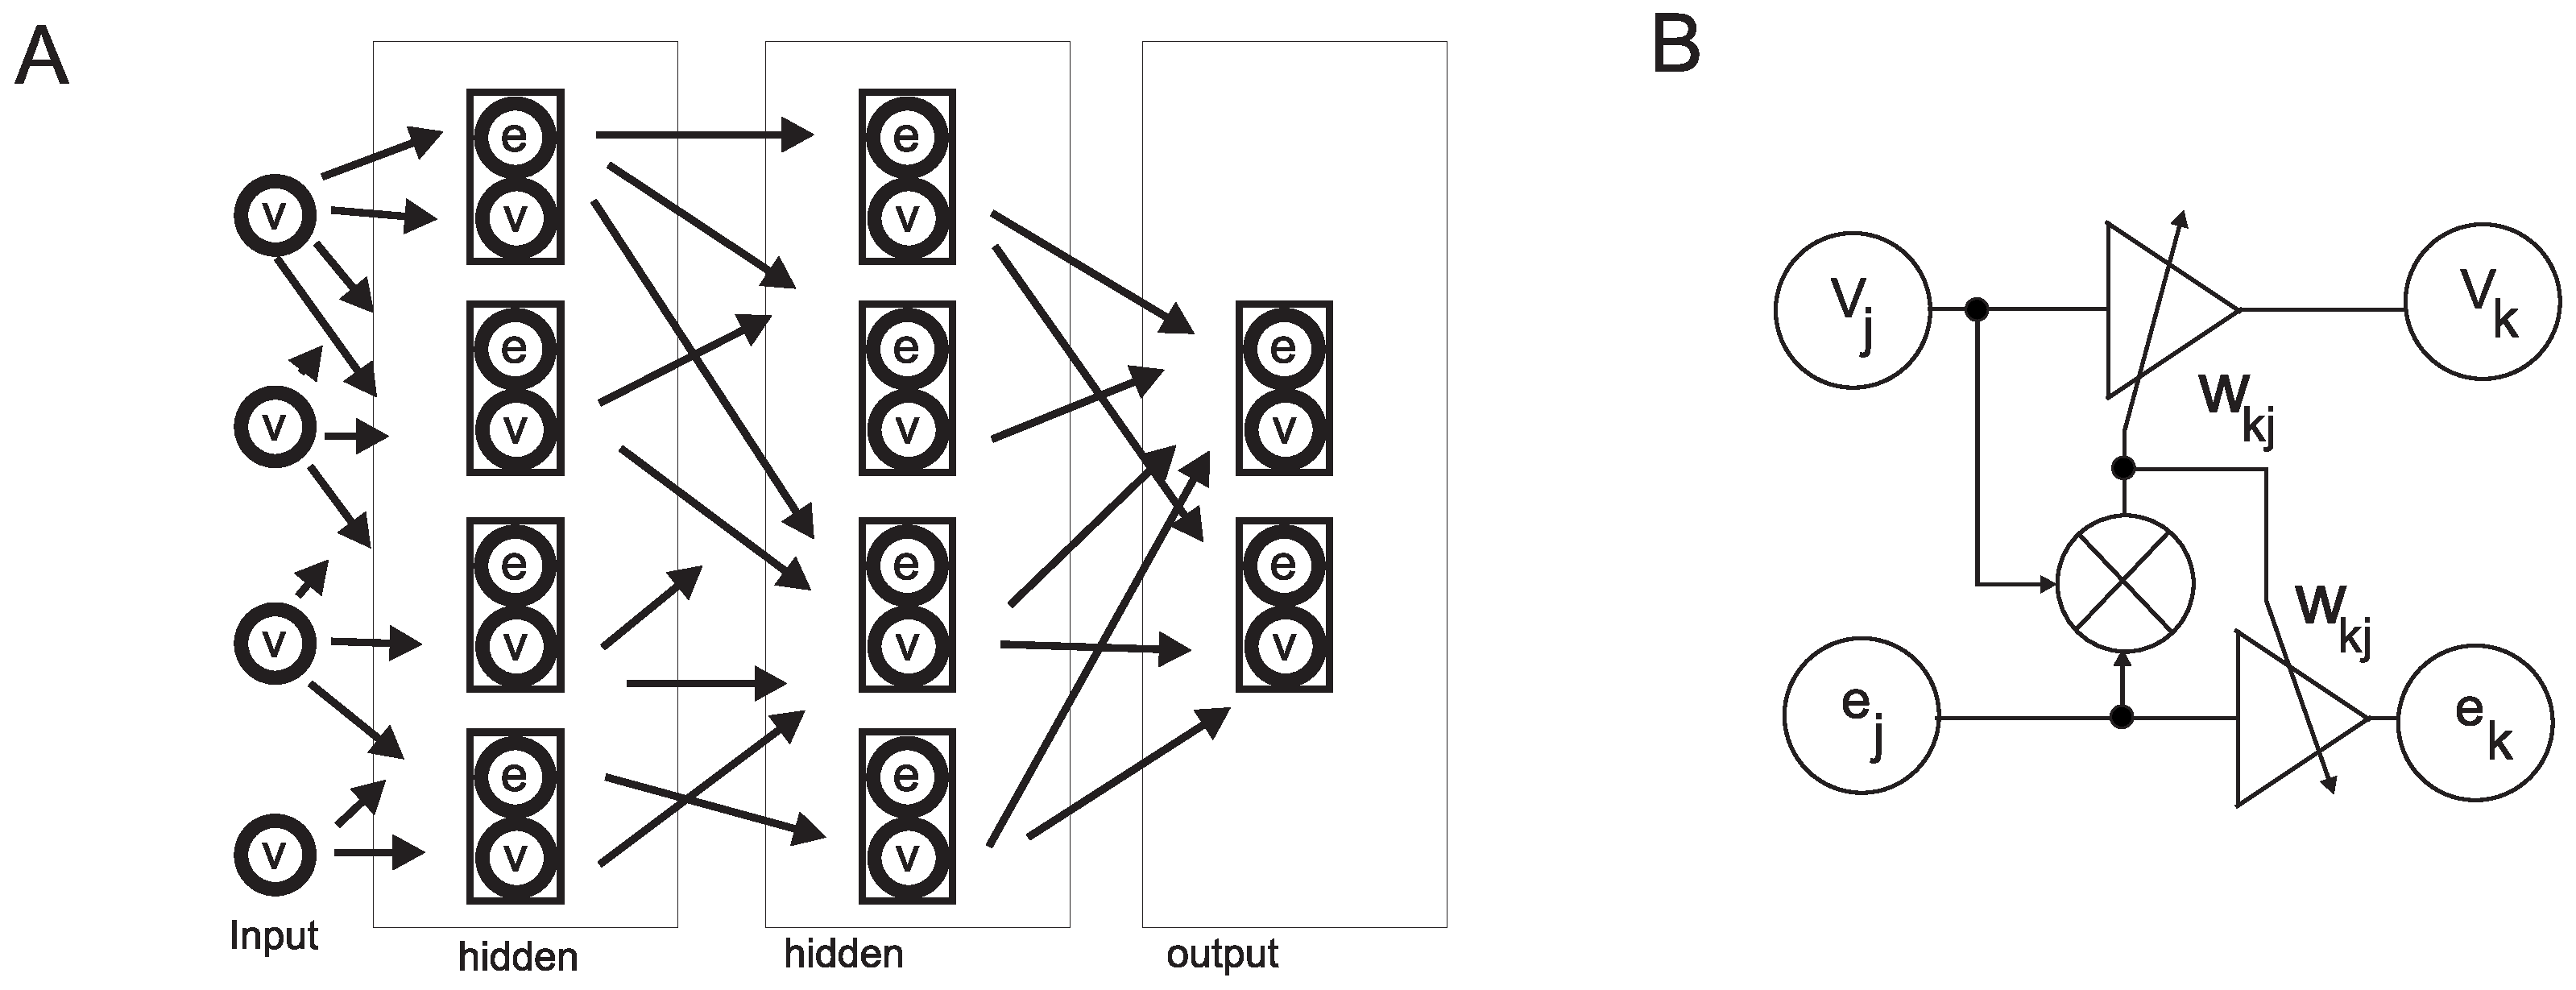
\includegraphics[width=\columnwidth]{netw_together}
  \caption{A) Overview of the network. Except for the input layer
    every neuron is a composite neuron with an activation $v$ and
    and an error term $e$. These are propagated through the network
    in a weighted fashion in parallel.
B) Computation in a single cell composite cell in the network.
    The presynaptic activities $v_k$ and error signals $e_k$ are used
    to perform correlation based learning and change the weight $w_{kj}$
    which weights both the activity and the error towards the next
    layer.\label{netw_together}}
\end{figure}


\section{Deep feedback learning}
We define a network with an input layer, hidden units and an output
layer which can all have different number of neurons (see
Fig~\ref{netw_together}A). However, in contrast to traditional
networks every layer (except for the input layer) consists of two
summation nodes: the actual activity and an error signal. These
are processed in two parallel streams.

Let us first focus on the calculation of the network activity and then
we deal with the error processing. We define a multi layered network
where every neuron is a standard computational unit which calculates
the weighted sums of its inputs and then sent through an activation
function:
\begin{equation}
  v_k = \Theta\left( \sum_i w_{jk} v_{j} \right)
\end{equation}
where the activity feeds from neurons in layer $v_j$ to neurons in layer $v_k$
and so forth. The activities are weighted by the weights $w_{jk}$
in a standard fashion.

The weight change is then calculated in a semi Hebbian fashion:
\begin{equation}
  w_{jk} = w_{jk} + \gamma v_j * e_k
\end{equation}
where $v_j$ is the presynaptic activity and $e_k$ is the error signal
attached to the postsynaptic neuron so that the correlation is
calculated between the input signals and the error signals. This is similar
to Hebbian learning but here the presynaptic term is the activity
and postsynaptic one is the error signal.

The error signal needs to be described in more detail how this
is propagated through the network. As described above the error
signal emerges from the feedback loop which is injected into the
network at its first hidden layer as the ``postsynaptic'' activity.
Since the 1st hidden layer directly receives its error signal this
can be computed instantly.

For the deeper layers the error signal is computed as a weighted
sum of the error signals from the previous layer:
\begin{equation}
  e_k = \frac{\left( \sum_j w_{jk} e_{j} \right) \Theta^\prime (v_k) }{\sqrt{\sum_j w_{jk}}}
\end{equation}
where the $\Theta^\prime (v_k)$ is the derivative of the activation
function $\Theta(v_k)$.

The computations performed in every layer are shown in
Fig~\ref{netw_together}B where we see that the activity $v_j$ is
weighted by the weight $w_{jk}$ and then summed up in the next
layer. The same happens for the error signal $v_j$ which is also
weighted by $w_{jk}$. Remember that for the 1st hidden layer this
error signal is just the injected error signal from the feedback loop
and is not the weighted sum.

Learning is then performed in three steps: first the activity is propagated through
the network, then the error signal is propagated via the same mechanism and then the
weights are adjusted. Thus, both the error
signal and the activity is propagated in a forward fashion through the network.
Learning itself is the ``Hebbian'' but by correlating the actual activation
and the error signal. 



\section{Results}

\section{Discussion}

\bibliographystyle{splncs03}

\bibliography{sab_submission,isab,ours}

\end{document}



\begin{figure}[h!]
  \centering
  \includegraphics[width=\columnwidth]{arena_cct.pdf}
  \caption{A. Overview of the simulation environment. The arena has two markers, labelled R and B (red and blue), within   \label{fig:cct}
    }
\end{figure}

